\section{The lens modeling challenge} \label{sec:results}

\subsection{\sw} \label{sec:SpaceWarps}
some words about \sw

\subsection{The simulated lenses} \label{sec:sims}

In order to estimate users performance, \sw included some simulated lensing configurations in their image set.

There are three kinds of simulated lenses.

Sims produced using {\tt gravlens}
\citep{2001astro.ph..2341K,2001astro.ph..2340K}.

\begin{itemize}
  \item {\em Quasar:\/} A singular elliptical isothermal plus constant
    external shear, with a circular Gaussian source.
  \item {\em Galaxy:\/} Lens as with quasar, but elliptical de
    Vaucouleurs source.
  \item {\em Galaxy:\/} Lens is circular NFW plus one dominant
    elliptical SIE and perturbating elliptical SIEs, source as with
    galaxy.
\end{itemize}

Singular isothermal is in equations (33-35) of
\cite{2001astro.ph..2341K} with core radius set to zero. NFW is
equations (48,50) of the same paper, and shear is the $\gamma$ term in
equation (76) of that work.




\subsection{The test setup} \label{sec:testsetup}

We made use of the simulated lenses (sims) to test the volunteers abilities to model those sims.

The testing was done with a small number of volunteers ($N_\text{v}=4$) and a set of simulated configurations ($N_\text{sim}=29$) chosen to represent some typical configurations.
The volunteers were given an introduction video explaining the theory behind gravitational lensing and the usage of \spl.
Additionally the volunteers had the opportunity to pose general questions to the experts during several hangouts during the training phase that preceded the modeling challenge.\footnote{No questions about the to be modeled sims were answered.}

To estimate the performance of the volunteers and the quality of the generated models, two test T1 and T2 were done.
%\begin{enumerate}
%  \item (T1) Correct identification of extremal points
%  \item (T2) Reproduction of the mass distribution of the lens
%\end{enumerate}

T1 tested the volunteers ability to reconstruct the arrival time surface given a survey image containing a sim.
This task consists of two parts.
First, the correct identification and location of lensed images (T1a).
Second to find the correct ordering in respect of the arrival time for the identified lensed images (T1b).

While we expected T1a to be trivial, given the nature of the survey images and the success of \sw, we expect T1b to pose more problems.
T1b tests the volunteers understandings of the theory of arrival time surfaces and the odd number theorem.
While we can provide the volunteers with some general rule of thumbs, T1b involves a lot of imagination and guessing and therefore a training effect could be visible in this test.

T1 was also designed to give some feedback on the difficulties volunteers encounter, to further imrove the tutorial materials.

The second test T2 was to compare the desired results of a modeling process, the mass distribution of the lens $\kappa(x, y)$.
To get a means of comparing the simulated data (sims) to the generated modeled data (models), the total convergence, also called enclosed mass $\kappa_{\text{encl}}(r)$ for both was calculated.
The Einstein radius $\Theta_E$ is defined by $\kappa_{\text{encl}}(\Theta_E)=1$ and gives a number that allows the comparison between the sims and the models.

\todo{!} Should I write down prior expectation for T2 too?




\subsection{First test T1} \label{sec:tests.t1}

The evaluation of the volunteers performance for T1 was done manually, comparing their input from \spl and the resulting reconstructed arrival time surface contour line plot (arrival plot) to the arrival plot genreated using simulation parameters.
\Figref{output_compare} shows the setup used to evaluate the models.

\begin{figure}
  \centering
  \subfigure{\includegraphics[width=0.45\textwidth]
             {fig/sims/006917/input.png}}
  \subfigure{\includegraphics[width=0.45\textwidth]
             {fig/sims/006917/spaghetti.png}} \\
  \subfigure{\includegraphics[width=0.45\textwidth]
             {fig/sims/ASW0001hpf/arriv.png}}
  \subfigure{\includegraphics[width=0.45\textwidth]
             {fig/sims/ASW0001hpf/extr_points.png}}
  \caption{Examples of Spaghetti input (left top) and modeled arrival time surface (right top) vs reconstructed arrival time surface from simulation parameters (bottom left), additionally using a extremal point detector (bottom right).
  \label{fig:output_compare}}
\end{figure}

To evaluate T1a and T1b, each model was evaluated with two binary tests.
The first is passed, if all the images have been identified and are approx. within $\pm0.05\cdot\text{imgwidth}$.
The second test is passed, if those identified points have the right parity, ordering with respect to arrival time.

Additionally, ten types of errors that could occur were analyzed, where each model could contain multiple of those.
The complete table with the results for each model can be found in the appendix, \tabref{detail_results}.

In \tabref{stats} a summary of this evaluation is presented.

%\begin{enumerate}
%1  \item inaccurate placement in an extended arc
%2  \item wrongly identified sad and min in 3 image configuration
%3  \item identified only 3 instead of 5 images
%4  \item tried to model an arc with a min instead of min-sad-min
%5  \item PI-err (rotation by 180 degrees; in 5 image configuration, exchanged the ordering of the two saddle points)
%6  \item PI/2-err (rotation by 90 degree; sad$\longmapsto$min$\longmapsto$sad$\longmapsto$min$\longmapsto$sad)
%7  \item missed faint image(s)
%8  \item tried to model an arc with min-sad-min instead of only min
%9  \item did identify two close by images as one
%10  \item used 7 or more image to model a 5 image system.
%\end{enumerate}

\input{tab/auto/_stats}


We conclude that the volunteers are performing very well identifying images and putting them approximately at the right spot (test 1), with a performance of 92\%.
Most of the problems where due to unclear arc-like structures (Error 1, p=0.18; Error 4, p=0.03; Error 8, p=0.04).
Critical failures like the failure to identify all fife images in an fife image system (Error 3, p=0.04) or to include too many images (Error 10, p=0.01) did almost never happend.
From this we conclude that the introduction materials was adequate and the volunteers got the basics of gravitational lensing.

\todo{add more detail?} Add more details like total amount of images detected / tot am images (rightPlace fraction)??


The ordering and assignment of minima / maxima / saddlepoint posed a more difficult task.
In p=59\% (N=70) of the cases the volunteers succeeded to identify the right configuration.
Most of the failures are due to error type 6 (PI/2), with N=38, p=32\%, followed by type 5 (PI) with N=7, p=6\%.
For an example of type 6 error, see \figref{6971}.










\subsection{Second test T2} \label{sec:results.2}

In \figref{eR_all} can be seen, that the calculated einstein radius $\Theta_E$ of the models tend to be too high.
The overshoot varies from around 0.2 to 0.4 for for good models.
One of the reasons for this is, that it's hard to get the center of the lens on spot.
An offset leads to a a flatter mass profile for the model compared to the simulation.



\begin{figure}[htbp]
  \centering
    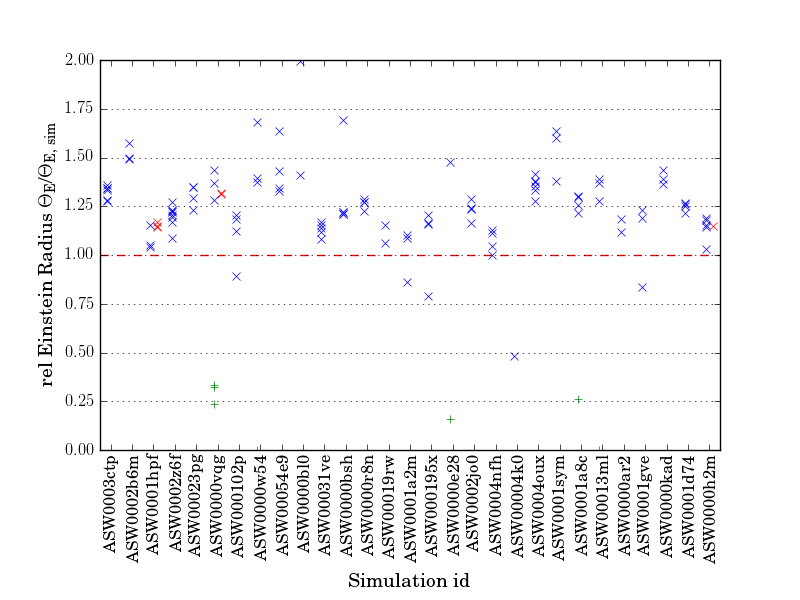
\includegraphics[width=0.80\textwidth]{fig/sims/eR_4.png}
  \caption{relative Einstein Radius for each model, per sim. }
  \label{fig:eR_all}
\end{figure}




\hr

Figure \ref{fig:6941} shows a simple example.

Figure \ref{fig:6975} shows an example where substructure introduces a
complication, but model ok.

Figure \ref{fig:6937} shows a case where substructure leads to a
poorer model.

Figure \ref{fig:6975} shows a nice symmetric quad.

Figure \ref{fig:6990} shows a long-axis quad.

Figure \ref{fig:6919} shows a short-axis quad.

Figure \ref{fig:6915} shows an inclined quad.

Figure \ref{fig:6971} shows incorrect identification, but the enclosed
mass still quite well recovered.




\clearpage
